\documentclass{homework}
\usepackage{marvosym}
\usepackage{hyperref}
\usepackage{color}

\course{Algorithmische Bioinformatik}
\semester{Wintersemester 2012 / 2013}
\no{8}
\date{Montag, dem 10. Dezember 2012}
\author{Stefan Meißner (4279113) und Niels Hoppe (4356370)}
\tutorial{Dienstag 08:00 - 10:00}
\tutor{Alena van Bömmel (Übungsgruppe 3)}

\begin{document}
\maketitle
\begin{enumerate} 

\aufgabe{Nussinov-Algorithmus}{80}

%Nussinov
%
%w(i,j) = score, max. Anz. Basenpaare für Subseqeunz x_i, ..., x_j
%\delta (i, j) = \begin{cases}
%1 & \text{ if } i \cdot j\\
%0 & \text{ else }
%\end{cases}
%
%Initialisierung
%w(i, i) = 0; w(i, i-1) = 0; i = 2, ..., L
%
%Rekursion
%alle Subsequenzen der Länge 2 ... L
%w(i, j) = \max \begin{cases}
%w(i+1, j)								& (1)\\
%w(i, j-1)								& (2)\\
%w(i+1, j-1) + \delta(i, j)				& (3)\\
%\max_{i < k < j} w(i, k) + w(k+1, j)	& (4)
%\end{cases}
%
%Traceback
%
%push(1, L)
%
%pop(i, j)
%if j \geq i: continue
%elif w(i+1,j) = w(i, j): push(i+1, j)
%elif w(i, i-1) = W[i, j]: push(i, j-1)
%elif W[i+1, j-1] + delta(i, j) = W[i, j]:
%	push(i+1, j-1)
%	print(i, j)
%else:
%	for k in range(i+1, j-1):
%		if W[i, k] + W[k+1, j] = W[i, j]:
%			push(i, k)
%			push(k+1, j)
%			break
%
%
%
%Information content IC von (P(X)M)_{PSSM}
%
%self-information - \log_2(P_{i,j})
%(avg) expected information -P_{i,j} \log_2(P{i,j}
%IC entropy - \sum_{i,j} P{i,j} \cdot \log_2(P_{i,j}) \Rightarrow (i)
%relative entropy \sum_{i,j} P_{i,j} \cdot \log_2(\frac{P_{i,j}}{P_B})
%f_{i,j](a,b) = H_{i,j} = - \sum_{a,b \in \mathcal{A}} f_{i,j}(a,b) \cdot \log_2 \frac{f_{i,j}(a,b)}{f_i(a) \cdot f_j(b)}
%Häufigkeit von Paar (a,b) in Spalten i und j
\begin{enumerate}
\item Das vorhandene Python Programm wurde an wenigen Stellen angepasst, um unseren Bedürfnissen gerecht zu werden. Um mit dem Fasta Format umgehen zu können, werden beim Einlesen der Sequenz alle Zeilen beginnend mit einem '$>$' Zeichen ausgelassen. 
Weiterhin müssen alle Zeilen zusammen als eine Sequenz behandelt werden.
\begin{verbatim}
seq=[]
stringSeq = ""

for line in f:
    # meta daten des fasta formats skippen
    if not line.startswith('>'):
        stringSeq += string.strip(line)
    # else: TODO: neue Sequenz zu seq hinzufuegen

seq.append(stringSeq)
\end{verbatim}
\item
Im Traceback Schritt muss beim Hinzufügen eines Basenpaares darauf geachtet werden, dass $i$ und $j$ einen Mindestabstand von 3 haben:
\begin{verbatim}
# auf hairpin loops >= 3 achten!
elif s[i,j]==s[i+1,j-1]+delta(seq[i],seq[j]) and j-i >= 3:
    pair.append([i,j,str(seq[i]),str(seq[j])]);
    traceback(s,seq,i+1,j-1,pair);
\end{verbatim}
Die angepasste Scoringfunction ist gegeben durch:
\begin{verbatim}
def delta(l,m):
    delta=0;
    if l=='A' and m=='U':
        return 2;
    elif l=='U' and m=='A':
        return 2;
    elif l=='G' and m=='C':
        return 3;
    elif l=='C' and m=='G':
        return 3;
    else:
        return 0;
\end{verbatim}

\item
Wir ersetzen alle 'T's durch ein 'U' durch:
\begin{verbatim}
seq = map(lambda x: str.replace(x, "T", "U"), seq)
\end{verbatim}

Das Programm liefert folgendes Ergebnis:
\begin{verbatim}
max # of folding pairs:  162
\end{verbatim}
\item 
Bracket- bzw. Vienna-Darstellung (Berechnung, siehe Quellcode).
\begin{verbatim}
0   ATGCCGTCCAAGGGCCCGCTGCAGTCTGTG
    .(()()(((.(((())())))(((.)))((
30  CAGGTCTTCGGACGCAAGAAGACAGCGACA
    )))(((((()(.()))))).(((.)()(((
60  GCTGTGGCGCACTGCAAACGCGGCAATGGT
    ())))(()()(((())..()()().()).)
90  CTCATCAAGGTGAACGGGCGGCCCCTGGAG
    )))()))).(((((().(((())((.))((
120 ATGATTGAGCCGCGCACGCTACAGTACAAG
    (((()(.)()(())))()(()(.(())(((
150 CTGCTGGAGCCAGTTCTGCTTCTCGGCAAG
    ))())))(()(.))))))))))(()())((
180 GAGCGATTTGCTGGTGTAGACATCCGTGTC
    ((.()()((()(((((()(((()(().)((
210 CGTGTAAAGGGTGGTGGTCACGTGGCCCAG
    ().(()((((((((.(((((())(())(.)
240 ATTTATGCTATCCGTCAGTCCATCTCCAAA
    ()((()()(()(()(.))(((()(((((((
270 GCCCTGGTGGCCTATTACCAGAAATATGTG
    ()((.)))(()))()()((.)..(()))))
300 GATGAGGCTTCCAAGAAGGAGATCAAAGAC
    )().))()((.(..))))))(())))))))
330 ATCCTCATCCAGTATGACCGGACCCTGCTG
    ())).)().(((()(.)(()(.)((.().)
360 GTAGCTGACCCTCGTCGCTGCGAGTCCAAA
    )())))))))))())(().)))))))))((
390 AAGTTTGGAGGCCCTGGTGCCCGCGCTCGC
    ((.)))(((.()((.)))())(()))))()
420 TACCAGAAATCCTACCGATAA
    ())(.))))))))))()()..
\end{verbatim}
Base Pair Graph, erzeugt mit der VARNA GUI:
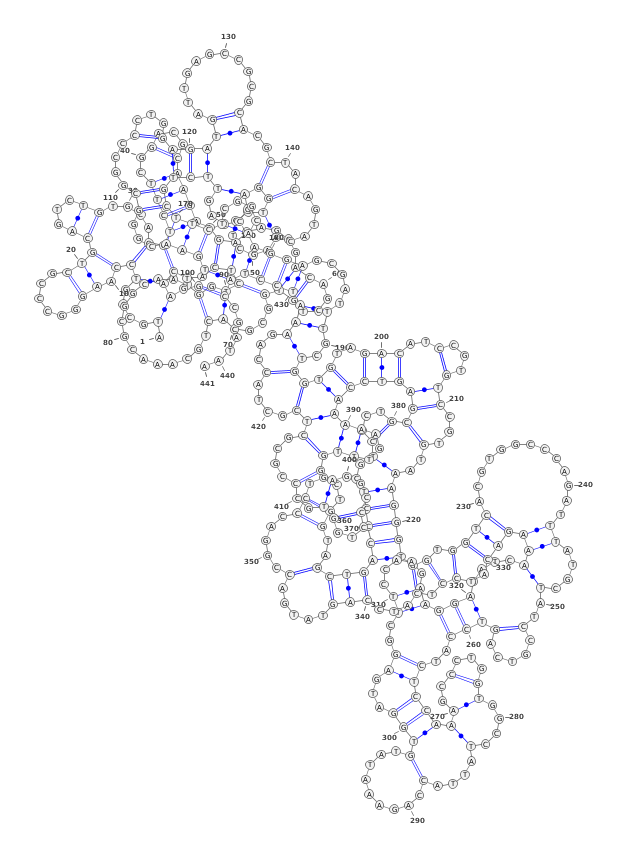
\includegraphics[scale=0.25]{../data/u8_aufg27_nussinov}

\item
\begin{verbatim}
RNAfold -p -d2 --noLP < rna16s.fa > zuker.out
\end{verbatim}

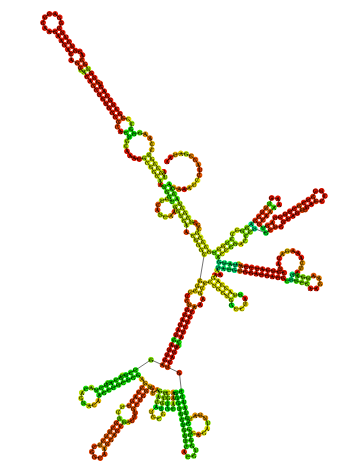
\includegraphics[scale=0.5]{../data/u8_aufg27_zuker_output}

\item
Der Nussinov-Algorithmus findet 199 (ohne Hairpin-Loop Restriktion) bzw. 162 Basenpaare. Der Basenpaar-Graph wirkt durch die vielen Loops sehr chaotisch. Beim Zuker Algorithmus werden 116 Basenpaare gefunden. 
Der Graph enthält viel weniger Loops und wirkt einfacher. 
Die Unterschiede sind auf die Biologische Relevanz zurückzuführen. Siehe Wikipedia Eintrag zum Nussinov-Algorithmus:\\
\textit{Die Sekundärstruktur, welche die maximale Anzahl von Basenpaaren enthält ist nicht unbedingt die Struktur, die in der Natur (in einer Zelle) auftritt. Deshalb wird in der Praxis der Nussinov-Algorithmus nicht zur Strukturvorhersage von RNA-Sequenzen eingesetzt. In der Praxis wird die Sekundärstruktur beispielsweise unter einem thermodynamischen Modell vorhergesagt, was zu biologisch sinnvolleren Ergebnissen führt.}

\end{enumerate}


\aufgabe{Entropie}{60}
\begin{itemize}
	\item
	\item
Zum Erzeugen der Sequenzen nutzen wir folgenden Converter:
\begin{verbatim}
#!/usr/bin/env python

import math
import csv
import sys

data = []
reader = csv.reader(open(sys.argv[1], "rb")) # TATA Box einlesen
for row in reader:
  row = list(int(elem) for elem in row)
  data.append(row)
  
multi_align = []
for x in range(389):
  multi_align.append("")

nukleotid = ['A','C','G','T']

for pos in range(len(data[0])):
  seq_index = 0
  for nuk in range(4): 
    val = data[nuk][pos]
    for i in range(val):
      multi_align[seq_index] += nukleotid[nuk]
      seq_index += 1
      
for seq in multi_align:
  print seq
\end{verbatim}

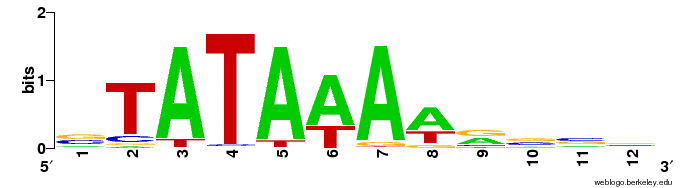
\includegraphics[scale=0.6]{../data/u8_aufg28b}
	\item
\begin{verbatim}
#!/usr/bin/env python
import math

# Spalte 1,2,3
f_i = [	[2,2,2], # A
        [2,2,1], # C
        [2,2,4], # G
        [2,2,1]] # U
f_ij = [[0,1,0], # AA
        [0,0,1], # AC
        [0,1,1], # AG
        [2,0,0], # AU
        [0,0,1], # CA
        [0,0,0], # ...
        [2,2,0],
        [0,0,1],
        [0,1,1], # GA
        [2,0,0],
        [0,0,2],
        [0,1,0],
        [2,0,1], # UA
        [0,1,0],
        [0,1,1],
        [0,0,0]] # UU

H = 0

for i in range(4):
  for j in range(4): 
    for spalte in range(3):
      p = f_ij[i*4+j][spalte]
      a = f_i[i][spalte]
      b = f_i[j][spalte]
      
      if p == 0:
        p = float(1)/16 # pseudocount
      else:
        p = float(p)/8
      
      a = float(a)/8
      b = float(b)/8
      
      H += p * math.log((p/(a*b)), 2)
      
print (-H) # -4.9375
\end{verbatim}	
	
\end{itemize}

\aufgabe{STS Content Mapping}{50}
\begin{enumerate}

\item Aus den Hamming-Distanzen der Sonden ergibt sich der linke Graph, indem wir den rechten MST berechnen:

\newpage

% \begin{verbatim}
%   ABCD     ABCD
% A  331   A    1
% B 3 22   B   22
% C 31 4   C  2
% D 124    D 12
% \end{verbatim}

\item Aus dem MST ergibt sich als kürzester Pfad mit Länge $5$ die Anordnung der Sonden als $(A,D,B,C)$:

\begin{tabular}{l|cccc}
	& A	& D	& B	& C\\\hline
1	& 1	& 1	& 1	& 0\\
2	& 1	& 1	& 0	& 0\\
3	& 0	& 0	& 1	& 1\\
4	& 1	& 0	& 0	& 1
\end{tabular}

\item Die Einträge $4A$ oder $4C$ widersprechen der C1P und sind darum wahrscheinlich fehlerhaft.

\end{enumerate}

\aufgabe{Gene finding (Übungsblatt 7)}{100}

Mit Hilfe der Funktion \texttt{train} erzeugen wir für jeden reading-frame ein eigenes Modell in Form einer Transitionsmatrix.
Zur besseren Lesbarkeit sind die Transitionsmatrizen jeweils mit $10^3$ skaliert dargestellt.

\begin{lstlisting}[language=python]
def train(seqs):
	nucs = ["a", "c", "g", "t"]
	binucs = list(itertools.product(nucs, repeat=2))
	trinucs = list(itertools.product(nucs, repeat=3))

	C = [dict([("".join(trinuc), 1.0) for trinuc in trinucs]) for i in range(3)]
	A = [dict([("".join(binuc),
		dict([("".join(binuc), 0.0) for binuc in binucs]))
		for binuc in binucs]) for i in range(3)]

	for seq in seqs:
		step = 0
		cod = seq[:3]			# current codon

		for nuc in seq:
			rfn = step % 3		# reading frame number is 0, 1 or 2
			C[rfn][cod] = C[rfn][cod] + 1
			step = step + 1;
			cod = cod[1:] + nuc

	for i in range(len(C)):
		for trinuc in C[i]:
			rs, st = trinuc[:2], trinuc[1:]
			A[i][rs][st] = C[i][trinuc] / sum([C[i][rs+l] for l in nucs])

	return (A[0], A[1], A[2])
\end{lstlisting}

\begin{enumerate}

\item Modell für \texttt{Genes.fa}

\tiny

\normalsize
reading-frame 1
\tiny

\begin{tabular}{c|cccccccccccccccc}
   & aa & ac & gt & ag & cc & ca & cg & gg & tt & gc & at & ga & tg & ta & tc & ct\\\hline
aa & 308 & 187 &   0 & 256 &   0 &   0 &   0 &   0 &   0 &   0 & 248 &   0 &   0 &   0 &   0 &   0\\
ac &   0 &   0 &   0 &   0 & 234 & 294 & 115 &   0 &   0 &   0 &   0 &   0 &   0 &   0 &   0 & 357\\
gt &   0 &   0 &   0 &   0 &   0 &   0 &   0 &   0 & 399 &   0 &   0 &   0 & 175 & 193 & 234 &   0\\
ag &   0 &   0 & 231 &   0 &   0 &   0 &   0 & 145 &   0 & 154 &   0 & 471 &   0 &   0 &   0 &   0\\
cc &   0 &   0 &   0 &   0 & 148 & 419 & 120 &   0 &   0 &   0 &   0 &   0 &   0 &   0 &   0 & 312\\
ca & 442 & 154 &   0 & 182 &   0 &   0 &   0 &   0 &   0 &   0 & 222 &   0 &   0 &   0 &   0 &   0\\
cg &   0 &   0 & 469 &   0 &   0 &   0 &   0 & 132 &   0 & 177 &   0 & 221 &   0 &   0 &   0 &   0\\
gg &   0 &   0 & 532 &   0 &   0 &   0 &   0 & 107 &   0 & 169 &   0 & 192 &   0 &   0 &   0 &   0\\
tt &   0 &   0 &   0 &   0 &   0 &   0 &   0 &   0 & 256 &   0 &   0 &   0 & 287 & 269 & 187 &   0\\
gc &   0 &   0 &   0 &   0 & 247 & 254 &  97 &   0 &   0 &   0 &   0 &   0 &   0 &   0 &   0 & 402\\
at &   0 &   0 &   0 &   0 &   0 &   0 &   0 &   0 & 346 &   0 &   0 &   0 & 256 & 178 & 220 &   0\\
ga & 374 & 175 &   0 & 150 &   0 &   0 &   0 &   0 &   0 &   0 & 301 &   0 &   0 &   0 &   0 &   0\\
tg &   0 &   0 & 338 &   0 &   0 &   0 &   0 & 401 &   0 & 213 &   0 &  48 &   0 &   0 &   0 &   0\\
ta &  21 & 452 &   0 &  15 &   0 &   0 &   0 &   0 &   0 &   0 & 512 &   0 &   0 &   0 &   0 &   0\\
tc &   0 &   0 &   0 &   0 & 229 & 277 & 120 &   0 &   0 &   0 &   0 &   0 &   0 &   0 &   0 & 374\\
ct &   0 &   0 &   0 &   0 &   0 &   0 &   0 &   0 & 287 &   0 &   0 &   0 & 258 & 313 & 141 &   0\\
\end{tabular}

\normalsize
reading-frame 2
\tiny

\begin{tabular}{c|cccccccccccccccc}
   & aa & ac & gt & ag & cc & ca & cg & gg & tt & gc & at & ga & tg & ta & tc & ct\\\hline
aa & 338 & 153 &   0 & 282 &   0 &   0 &   0 &   0 &   0 &   0 & 226 &   0 &   0 &   0 &   0 &   0\\
ac &   0 &   0 &   0 &   0 & 156 & 354 & 266 &   0 &   0 &   0 &   0 &   0 &   0 &   0 &   0 & 225\\
gt &   0 &   0 &   0 &   0 &   0 &   0 &   0 &   0 & 194 &   0 &   0 &   0 & 355 & 322 & 128 &   0\\
ag &   0 &   0 & 200 &   0 &   0 &   0 &   0 & 279 &   0 & 182 &   0 & 340 &   0 &   0 &   0 &   0\\
cc &   0 &   0 &   0 &   0 & 124 & 452 & 222 &   0 &   0 &   0 &   0 &   0 &   0 &   0 &   0 & 202\\
ca & 330 & 171 &   0 & 259 &   0 &   0 &   0 &   0 &   0 &   0 & 240 &   0 &   0 &   0 &   0 &   0\\
cg &   0 &   0 & 222 &   0 &   0 &   0 &   0 & 255 &   0 & 194 &   0 & 330 &   0 &   0 &   0 &   0\\
gg &   0 &   0 & 250 &   0 &   0 &   0 &   0 & 244 &   0 & 175 &   0 & 331 &   0 &   0 &   0 &   0\\
tt &   0 &   0 &   0 &   0 &   0 &   0 &   0 &   0 & 245 &   0 &   0 &   0 & 335 & 248 & 171 &   0\\
gc &   0 &   0 &   0 &   0 & 161 & 372 & 238 &   0 &   0 &   0 &   0 &   0 &   0 &   0 &   0 & 230\\
at &   0 &   0 &   0 &   0 &   0 &   0 &   0 &   0 & 224 &   0 &   0 &   0 & 326 & 298 & 152 &   0\\
ga & 383 & 139 &   0 & 253 &   0 &   0 &   0 &   0 &   0 &   0 & 226 &   0 &   0 &   0 &   0 &   0\\
tg &   0 &   0 & 170 &   0 &   0 &   0 &   0 & 300 &   0 & 153 &   0 & 377 &   0 &   0 &   0 &   0\\
ta & 308 & 194 &   0 & 262 &   0 &   0 &   0 &   0 &   0 &   0 & 237 &   0 &   0 &   0 &   0 &   0\\
tc &   0 &   0 &   0 &   0 & 167 & 415 & 224 &   0 &   0 &   0 &   0 &   0 &   0 &   0 &   0 & 194\\
ct &   0 &   0 &   0 &   0 &   0 &   0 &   0 &   0 & 231 &   0 &   0 &   0 & 319 & 282 & 168 &   0\\
\end{tabular}

\normalsize
reading-frame 3
\tiny

\begin{tabular}{c|cccccccccccccccc}
   & aa & ac & gt & ag & cc & ca & cg & gg & tt & gc & at & ga & tg & ta & tc & ct\\\hline
aa & 387 & 181 &   0 & 198 &   0 &   0 &   0 &   0 &   0 &   0 & 235 &   0 &   0 &   0 &   0 &   0\\
ac &   0 &   0 &   0 &   0 & 284 & 361 & 100 &   0 &   0 &   0 &   0 &   0 &   0 &   0 &   0 & 255\\
gt &   0 &   0 &   0 &   0 &   0 &   0 &   0 &   0 & 442 &   0 &   0 &   0 & 108 & 184 & 266 &   0\\
ag &   0 &   0 & 190 &   0 &   0 &   0 &   0 & 187 &   0 & 192 &   0 & 431 &   0 &   0 &   0 &   0\\
cc &   0 &   0 &   0 &   0 & 252 & 416 &  97 &   0 &   0 &   0 &   0 &   0 &   0 &   0 &   0 & 236\\
ca & 383 & 193 &   0 & 181 &   0 &   0 &   0 &   0 &   0 &   0 & 243 &   0 &   0 &   0 &   0 &   0\\
cg &   0 &   0 & 204 &   0 &   0 &   0 &   0 & 206 &   0 & 185 &   0 & 405 &   0 &   0 &   0 &   0\\
gg &   0 &   0 & 194 &   0 &   0 &   0 &   0 & 156 &   0 & 223 &   0 & 427 &   0 &   0 &   0 &   0\\
tt &   0 &   0 &   0 &   0 &   0 &   0 &   0 &   0 & 423 &   0 &   0 &   0 & 103 & 154 & 320 &   0\\
gc &   0 &   0 &   0 &   0 & 252 & 388 & 107 &   0 &   0 &   0 &   0 &   0 &   0 &   0 &   0 & 253\\
at &   0 &   0 &   0 &   0 &   0 &   0 &   0 &   0 & 416 &   0 &   0 &   0 & 109 & 168 & 307 &   0\\
ga & 413 & 161 &   0 & 162 &   0 &   0 &   0 &   0 &   0 &   0 & 264 &   0 &   0 &   0 &   0 &   0\\
tg &   0 &   0 & 206 &   0 &   0 &   0 &   0 & 192 &   0 & 216 &   0 & 386 &   0 &   0 &   0 &   0\\
ta & 361 & 212 &   0 & 141 &   0 &   0 &   0 &   0 &   0 &   0 & 286 &   0 &   0 &   0 &   0 &   0\\
tc &   0 &   0 &   0 &   0 & 294 & 380 &  92 &   0 &   0 &   0 &   0 &   0 &   0 &   0 &   0 & 234\\
ct &   0 &   0 &   0 &   0 &   0 &   0 &   0 &   0 & 414 &   0 &   0 &   0 & 118 & 176 & 292 &   0\\
\end{tabular}

\normalsize

\item Modell für \texttt{Noncoding.fa}

reading-frame 1
\tiny

\begin{tabular}{c|cccccccccccccccc}
   & aa & ac & gt & ag & cc & ca & cg & gg & tt & gc & at & ga & tg & ta & tc & ct\\\hline
aa & 385 & 172 &   0 & 182 &   0 &   0 &   0 &   0 &   0 &   0 & 260 &   0 &   0 &   0 &   0 &   0\\
ac &   0 &   0 &   0 &   0 & 258 & 303 & 151 &   0 &   0 &   0 &   0 &   0 &   0 &   0 &   0 & 288\\
gt &   0 &   0 &   0 &   0 &   0 &   0 &   0 &   0 & 353 &   0 &   0 &   0 & 185 & 233 & 229 &   0\\
ag &   0 &   0 & 236 &   0 &   0 &   0 &   0 & 181 &   0 & 199 &   0 & 383 &   0 &   0 &   0 &   0\\
cc &   0 &   0 &   0 &   0 & 225 & 351 & 115 &   0 &   0 &   0 &   0 &   0 &   0 &   0 &   0 & 310\\
ca & 380 & 194 &   0 & 161 &   0 &   0 &   0 &   0 &   0 &   0 & 266 &   0 &   0 &   0 &   0 &   0\\
cg &   0 &   0 & 266 &   0 &   0 &   0 &   0 & 206 &   0 & 214 &   0 & 314 &   0 &   0 &   0 &   0\\
gg &   0 &   0 & 258 &   0 &   0 &   0 &   0 & 182 &   0 & 201 &   0 & 360 &   0 &   0 &   0 &   0\\
tt &   0 &   0 &   0 &   0 &   0 &   0 &   0 &   0 & 409 &   0 &   0 &   0 & 190 & 148 & 254 &   0\\
gc &   0 &   0 &   0 &   0 & 254 & 307 & 135 &   0 &   0 &   0 &   0 &   0 &   0 &   0 &   0 & 305\\
at &   0 &   0 &   0 &   0 &   0 &   0 &   0 &   0 & 340 &   0 &   0 &   0 & 153 & 308 & 198 &   0\\
ga & 421 & 151 &   0 & 142 &   0 &   0 &   0 &   0 &   0 &   0 & 286 &   0 &   0 &   0 &   0 &   0\\
tg &   0 &   0 & 283 &   0 &   0 &   0 &   0 & 203 &   0 & 201 &   0 & 313 &   0 &   0 &   0 &   0\\
ta & 317 & 197 &   0 & 147 &   0 &   0 &   0 &   0 &   0 &   0 & 338 &   0 &   0 &   0 &   0 &   0\\
tc &   0 &   0 &   0 &   0 & 247 & 273 & 139 &   0 &   0 &   0 &   0 &   0 &   0 &   0 &   0 & 341\\
ct &   0 &   0 &   0 &   0 &   0 &   0 &   0 &   0 & 442 &   0 &   0 &   0 & 155 & 169 & 234 &   0\\
\end{tabular}

\normalsize
reading-frame 2
\tiny

\begin{tabular}{c|cccccccccccccccc}
   & aa & ac & gt & ag & cc & ca & cg & gg & tt & gc & at & ga & tg & ta & tc & ct\\\hline
aa & 387 & 183 &   0 & 181 &   0 &   0 &   0 &   0 &   0 &   0 & 249 &   0 &   0 &   0 &   0 &   0\\
ac &   0 &   0 &   0 &   0 & 245 & 309 & 166 &   0 &   0 &   0 &   0 &   0 &   0 &   0 &   0 & 281\\
gt &   0 &   0 &   0 &   0 &   0 &   0 &   0 &   0 & 327 &   0 &   0 &   0 & 246 & 256 & 171 &   0\\
ag &   0 &   0 & 269 &   0 &   0 &   0 &   0 & 201 &   0 & 202 &   0 & 328 &   0 &   0 &   0 &   0\\
cc &   0 &   0 &   0 &   0 & 196 & 342 & 156 &   0 &   0 &   0 &   0 &   0 &   0 &   0 &   0 & 307\\
ca & 379 & 176 &   0 & 186 &   0 &   0 &   0 &   0 &   0 &   0 & 260 &   0 &   0 &   0 &   0 &   0\\
cg &   0 &   0 & 327 &   0 &   0 &   0 &   0 & 172 &   0 & 236 &   0 & 265 &   0 &   0 &   0 &   0\\
gg &   0 &   0 & 332 &   0 &   0 &   0 &   0 & 182 &   0 & 212 &   0 & 274 &   0 &   0 &   0 &   0\\
tt &   0 &   0 &   0 &   0 &   0 &   0 &   0 &   0 & 365 &   0 &   0 &   0 & 214 & 196 & 225 &   0\\
gc &   0 &   0 &   0 &   0 & 219 & 335 & 165 &   0 &   0 &   0 &   0 &   0 &   0 &   0 &   0 & 280\\
at &   0 &   0 &   0 &   0 &   0 &   0 &   0 &   0 & 301 &   0 &   0 &   0 & 189 & 302 & 208 &   0\\
ga & 388 & 164 &   0 & 176 &   0 &   0 &   0 &   0 &   0 &   0 & 273 &   0 &   0 &   0 &   0 &   0\\
tg &   0 &   0 & 282 &   0 &   0 &   0 &   0 & 219 &   0 & 209 &   0 & 291 &   0 &   0 &   0 &   0\\
ta & 302 & 188 &   0 & 126 &   0 &   0 &   0 &   0 &   0 &   0 & 384 &   0 &   0 &   0 &   0 &   0\\
tc &   0 &   0 &   0 &   0 & 219 & 284 & 144 &   0 &   0 &   0 &   0 &   0 &   0 &   0 &   0 & 353\\
ct &   0 &   0 &   0 &   0 &   0 &   0 &   0 &   0 & 342 &   0 &   0 &   0 & 191 & 247 & 219 &   0\\
\end{tabular}

\normalsize
reading-frame 3
\tiny

\begin{tabular}{c|cccccccccccccccc}
   & aa & ac & gt & ag & cc & ca & cg & gg & tt & gc & at & ga & tg & ta & tc & ct\\\hline
aa & 378 & 156 &   0 & 207 &   0 &   0 &   0 &   0 &   0 &   0 & 259 &   0 &   0 &   0 &   0 &   0\\
ac &   0 &   0 &   0 &   0 & 206 & 329 & 210 &   0 &   0 &   0 &   0 &   0 &   0 &   0 &   0 & 255\\
gt &   0 &   0 &   0 &   0 &   0 &   0 &   0 &   0 & 318 &   0 &   0 &   0 & 221 & 297 & 164 &   0\\
ag &   0 &   0 & 245 &   0 &   0 &   0 &   0 & 217 &   0 & 192 &   0 & 345 &   0 &   0 &   0 &   0\\
cc &   0 &   0 &   0 &   0 & 207 & 388 & 126 &   0 &   0 &   0 &   0 &   0 &   0 &   0 &   0 & 279\\
ca & 344 & 206 &   0 & 185 &   0 &   0 &   0 &   0 &   0 &   0 & 265 &   0 &   0 &   0 &   0 &   0\\
cg &   0 &   0 & 337 &   0 &   0 &   0 &   0 & 172 &   0 & 199 &   0 & 292 &   0 &   0 &   0 &   0\\
gg &   0 &   0 & 296 &   0 &   0 &   0 &   0 & 197 &   0 & 186 &   0 & 321 &   0 &   0 &   0 &   0\\
tt &   0 &   0 &   0 &   0 &   0 &   0 &   0 &   0 & 398 &   0 &   0 &   0 & 201 & 220 & 180 &   0\\
gc &   0 &   0 &   0 &   0 & 181 & 306 & 173 &   0 &   0 &   0 &   0 &   0 &   0 &   0 &   0 & 339\\
at &   0 &   0 &   0 &   0 &   0 &   0 &   0 &   0 & 300 &   0 &   0 &   0 & 209 & 324 & 166 &   0\\
ga & 393 & 159 &   0 & 181 &   0 &   0 &   0 &   0 &   0 &   0 & 267 &   0 &   0 &   0 &   0 &   0\\
tg &   0 &   0 & 264 &   0 &   0 &   0 &   0 & 246 &   0 & 188 &   0 & 303 &   0 &   0 &   0 &   0\\
ta & 267 & 205 &   0 & 183 &   0 &   0 &   0 &   0 &   0 &   0 & 346 &   0 &   0 &   0 &   0 &   0\\
tc &   0 &   0 &   0 &   0 & 208 & 313 & 122 &   0 &   0 &   0 &   0 &   0 &   0 &   0 &   0 & 357\\
ct &   0 &   0 &   0 &   0 &   0 &   0 &   0 &   0 & 352 &   0 &   0 &   0 & 219 & 222 & 207 &   0\\
\end{tabular}

\normalsize

\item

Die Funktion \texttt{analyze} schiebt ein Fenster über die Sequenz und berechnet an jeder Position die Werte für $S$.
Um die Funktion \texttt{Pr} einzeln implementieren zu können, verwenden wir die Gleichung
$$\sum \log \frac{a}{b} = \sum \log a - \sum \log b.$$

\begin{lstlisting}[language=python]
def Pr(seq, A):
	return sum([math.log(A[seq[n:n+2]][seq[n+1:n+3]]) for n in range(0, len(seq)-3)])

def analyze(seq, Gmod, NCmod, winsize):
	data = []
	S = [0.0, 0.0, 0.0]

	step = 0
	win = seq[:winsize]		# current window

	for n in seq[winsize:]:
		rfn = step % 3		# reading frame number is 0, 1 or 2
		S[rfn] = Pr(win, Gmod) - Pr(win, NCmod)

		if rfn == 2:
			data.append((step, S[0], S[1], S[2]))

		step = step + 1;
		win = win[1:] + n
	return data
\end{lstlisting}

\item
\item

\end{enumerate}



\end{enumerate}
\end{document}
